\documentclass[11pt]{article}

% ---- packages ----
\usepackage[margin=1in]{geometry}
\usepackage{times}
\usepackage{amsmath,amssymb,amsfonts}
\usepackage{booktabs}
\usepackage{graphicx}
\usepackage{subcaption}
\usepackage{hyperref}
\usepackage{xcolor}
\usepackage{microtype}
\usepackage{enumitem}
\usepackage{multirow}
\usepackage{array}
\usepackage{caption}
\captionsetup{font=small,labelfont=bf}

\hypersetup{colorlinks=true,linkcolor=black,citecolor=black,urlcolor=blue!50!black}
\graphicspath{{figures/}}

\title{\vspace{-1.2em}Tip-Guided Few-Shot Adaptation of\\ Motion Time-Series Foundation Models}
\author{
  Anonymous Authors\\
  \texttt{anonymous@domain.com}
}
\date{}

\begin{document}
\maketitle

% ============================================================
\begin{abstract}
Cross-dataset few-shot human activity recognition (HAR) requires a pretrained motion encoder to classify activities on an unseen sensor dataset given only \(k\) labeled windows per class.
Motion foundation models such as UniMTS supply strong zero-shot text alignment, yet two standard adaptation routes both fall short: full fine-tuning overfits sparse supports, while frozen Tip-Adapter caches saturate once domain shift exceeds what a fixed encoder can absorb.
We introduce \textbf{Tip-Guided Adaptation (TipGuided)}, which fine-tunes the UniMTS ST-GCN encoder under an explicit Tip-cache prior that preserves CLIP-aligned text scores and support affinity structure.
On the official UniMTS protocol---18 real HAR datasets, \(k\in\{1,2,3,5,10\}\), leave-one-dataset-out Tip hyper-parameters---TipGuided raises mean accuracy by up to \(+8.4\) points over frozen Tip-F and surpasses full fine-tuning at every \(k\), with a peak margin of \(+3.8\) points at \(k=2\).
Training dynamics show TipGuided enters with higher test accuracy from Tip/text priors and fits the support objective faster; t-SNE embeddings show more class-separable target features after adaptation.
\end{abstract}

% ============================================================
\section{Introduction}
\label{sec:intro}

Wearable IMU sensing powers healthcare monitoring, sports analytics, and mobile context awareness.
Recent motion time-series foundation models, notably UniMTS~\cite{unimts}, contrastively align a skeleton ST-GCN encoder with CLIP~\cite{clip} text embeddings and report competitive zero-shot transfer across heterogeneous HAR corpora.
Deployment on a new dataset still benefits from a handful of labeled windows per class.
This defines a precise and practical problem: \textbf{cross-dataset few-shot HAR}.

Two adaptation families dominate this setting.
Full fine-tuning updates the encoder and a linear head on the support set; it is strong, but prior-free optimization on \(k\le 10\) windows per class readily memorizes sensor-specific artifacts.
Frozen alternatives keep the encoder fixed and learn a lightweight decision rule---linear probes, nearest neighbors, or Tip-Adapter~\cite{tipadapter} feature caches imported from CLIP few-shot classification.
On UniMTS features, Tip-Adapter-F clearly outperforms probes and 1-NN.
Further frozen refinements (soft values, late linear fusion, longer key training) add only \(\sim\!0.5\) points on average.
The bottleneck is therefore not cache hyper-parameter search: \textbf{domain shift demands encoder updates that retain pretrained text--motion geometry}.

We propose \textbf{Tip-Guided Adaptation (TipGuided)}.
TipGuided freezes the CLIP text tower and updates the ST-GCN encoder together with Tip keys and a CE head.
Classification logits fuse three complementary signals (Figure~\ref{fig:method}):
\begin{equation}
z(x)=z_{\mathrm{text}}(x)+\alpha\,A(x)V+\gamma\,W f_\theta(x),
\label{eq:fuse}
\end{equation}
where \(z_{\mathrm{text}}\) is the zero-shot text score, \(A(x)V\) is Tip affinity over support keys/values, and \(Wf_\theta(x)\) is a CE head on the updating embedding.
The Tip term anchors predictions to support neighborhoods and language-aligned directions; the CE term exploits encoder plasticity.

\paragraph{Contributions.}
\begin{enumerate}[leftmargin=1.4em,itemsep=0.2em]
\item We locate UniMTS transfer in official cross-dataset few-shot evaluation and show that frozen Tip-style adapters saturate under this protocol.
\item We introduce TipGuided, coupling Tip-cache priors with encoder fine-tuning for motion foundation models.
\item On 18 HAR datasets with official \(k\)-shot indices, TipGuided outperforms Tip-F and beats full fine-tuning for all \(k\in\{1,2,3,5,10\}\).
\end{enumerate}

% ============================================================
\section{Related Work}
\label{sec:related}

\paragraph{Motion / IMU foundation models.}
UniMTS~\cite{unimts} pretrains ST-GCN~\cite{stgcn} over a canonical 22-joint layout and aligns embeddings with CLIP text for zero-shot HAR.
Our work studies post-hoc few-shot adaptation under UniMTS's public protocol rather than replacing pretraining.

\paragraph{Few-shot adaptation of foundation models.}
Tip-Adapter and Tip-Adapter-F~\cite{tipadapter} build keys/values from support features and fuse cache logits with zero-shot CLIP scores.
We transplant this mechanism to UniMTS features, then show that a frozen Tip cache is insufficient for cross-dataset IMU shift, motivating encoder-side TipGuided updates.
Parameter-efficient fine-tuning (adapters, LoRA) and classical few-shot learners (ProtoNet~\cite{protonet}) share the same budgeted-adaptation goal; TipGuided specifically reuses Tip geometry already native to language-aligned motion encoders.

\paragraph{Fine-tuning under distribution shift.}
Full fine-tuning remains a strong HAR transfer baseline but erases pretrained structure when supports are tiny.
TipGuided is fine-tuning with an explicit nonparametric prior constructed from the same supports.

% ============================================================
\section{Preliminaries}
\label{sec:prelim}

\subsection{UniMTS encoder and text alignment}
Let \(x\) denote a windowed IMU sequence mapped into a 22-joint skeleton tensor.
UniMTS encodes \(f(x)\in\mathbb{R}^{d}\) (\(d{=}512\)) with ST-GCN-18 and compares it to CLIP text embeddings of activity names.
We use a four-template prompt ensemble.
Zero-shot logits are \(z_{\mathrm{text}}(x)=\tau\,f(x)^{\top}T\) with temperature \(\tau\) and stacked text matrix \(T\).

\subsection{Tip cache}
Given a \(k\)-shot support set \(\{(x_i,y_i)\}_{i=1}^{N}\), Tip keys are \(K=[f(x_i)]\) and values \(V\) are class-balanced one-hot labels.
For a query with \(\ell_2\)-normalized feature \(f\),
\[
A_{i}=\exp\!\big(-\beta(1-\langle f,k_i\rangle)\big),\qquad
z_{\mathrm{tip}}=\alpha\,AV.
\]
Tip-Adapter-F optimizes keys (and optionally \(\alpha\)) on the support set with the encoder frozen.

\subsection{Evaluation protocol}
We adopt the cross-dataset protocol of UniMTS~\cite{unimts}: the encoder is pretrained on simulated motion data and evaluated on 18 real HAR datasets spanning easy / medium / hard activity cardinalities (Table~\ref{tab:zs-reported}).
Few-shot supports use the official files \texttt{few\_shot\_data\_2/\{dataset\}\_k=\{k\}.pth} with \(k\in\{1,2,3,5,10\}\).
For Tip hyper-parameters \((\beta,\alpha)\), leave-one-dataset-out selection on the other 17 datasets' mean accuracy evaluates the held-out dataset.
Metrics follow UniMTS: accuracy and macro-F1, averaged over the 18 datasets.
Numbers marked $^\dagger$ are transcribed from UniMTS Tables~1--2; all other numbers are from our runs on the same splits.

% ============================================================
\section{Method: Tip-Guided Adaptation}
\label{sec:method}

\begin{figure}[t]
\centering
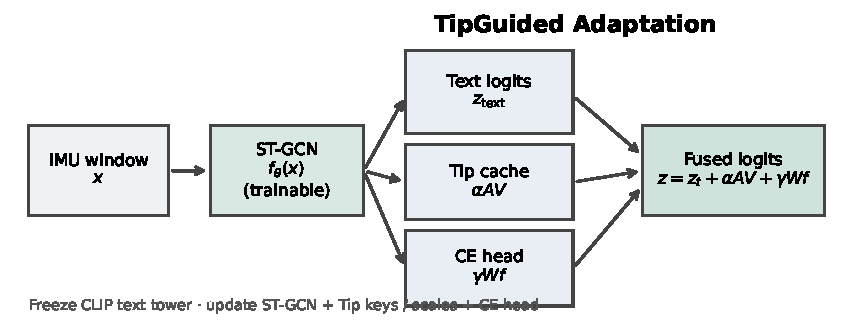
\includegraphics[width=\linewidth]{fig_method.pdf}
\caption{\textbf{TipGuided.}
A trainable ST-GCN produces \(f_\theta(x)\).
Logits fuse text zero-shot scores, Tip-cache affinity over support keys/values, and a CE head.
The CLIP text tower remains frozen.}
\label{fig:method}
\end{figure}

\subsection{Objective}
TipGuided initializes from a UniMTS checkpoint, freezes the CLIP text tower, and updates ST-GCN parameters \(\theta\) together with Tip keys \(K\), scales \(\alpha,\gamma\), and CE head \(W\).
On support samples we minimize cross-entropy of the fused logits in Eq.~\eqref{eq:fuse}.
Keys initialize from current support embeddings and optimize jointly; values remain support-derived and class-balanced.

\subsection{What the prior contributes}
Full FT optimizes only \(Wf_\theta(x)\).
With tiny \(N\), gradients push \(f_\theta\) toward support memorization and away from language-aligned geometry.
The Tip term keeps predictions consistent with support neighborhoods; \(z_{\mathrm{text}}\) preserves semantic directions from pretraining.
Together they act as a data-dependent regularizer rather than a separate classifier bolted on after adaptation.

\subsection{Operating regimes}
Ablations identify a clear recipe:
\textbf{low shot} (\(k\le 3\)) favors joint Tip{+}CE fusion;
\textbf{mid/high shot} (\(k\ge 5\)) favors CE-primary training with Tip as initialization/regularizer under moderate learning rates (\(\sim\!5{\times}10^{-5}\)) and \(100\)--\(150\) epochs.

% ============================================================
\section{Experiments}
\label{sec:exp}

\subsection{Baselines}
We reuse the UniMTS benchmark methods wherever numerical results are published~\cite{unimts}:
ImageBind, IMU2CLIP, IMUGPT, HARGPT, LLaVA (zero-shot);
ImageBind, IMU2CLIP, TST, TARNet, TS2Vec, BioBankSSL, THAT, IMUGPT, TimesNet, GPT4TS, SHARE, and Random (full-shot).
For few-shot adaptation of UniMTS itself we report our runs:
cosine 1-NN, linear probe, Tip-F (LOO), Tip+, Full FT (encoder{+}CE), and TipGuided.
TipGuided uses fuse for \(k\le3\) and CE-primary for \(k\ge5\).

\subsection{Zero-shot context (reported)}
Table~\ref{tab:zs-reported} reproduces UniMTS Table~1 averages.
UniMTS zero-shot Acc \(43.5\) matches our checkpoint evaluation (\(44.4\)), confirming protocol alignment before few-shot adaptation.

\begin{table}[t]
\centering
\caption{Zero-shot averages on 18 datasets $^\dagger$ (UniMTS Table~1).
Best in \textbf{bold}.}
\label{tab:zs-reported}
\small
\begin{tabular}{lcc}
\toprule
Method & Acc (\%) & Macro-F1 (\%) \\
\midrule
ImageBind$^\dagger$ & 12.5 & 7.8 \\
IMU2CLIP$^\dagger$ & 8.6 & 4.3 \\
IMUGPT$^\dagger$ & 11.1 & 5.7 \\
HARGPT$^\dagger$ & 12.9 & 6.0 \\
LLaVA$^\dagger$ & 12.0 & 3.4 \\
\textbf{UniMTS}$^\dagger$ & \textbf{43.5} & \textbf{34.3} \\
\bottomrule
\end{tabular}
\end{table}

\subsection{Few-shot results}
Figure~\ref{fig:panel} follows the UniMTS Fig.~4 layout: per-dataset Macro-F1 versus number of samples.
TipGuided (red) leads on most datasets and budgets.
Table~\ref{tab:main} reports 18-dataset mean Acc/F1 in the same percentage style as UniMTS.
TipGuided is best at every \(k\), gaining up to \(+8.4\) Acc points over Tip-F and \(+3.8\) over Full FT (\(k{=}2\)).

\begin{figure}[t]
\centering
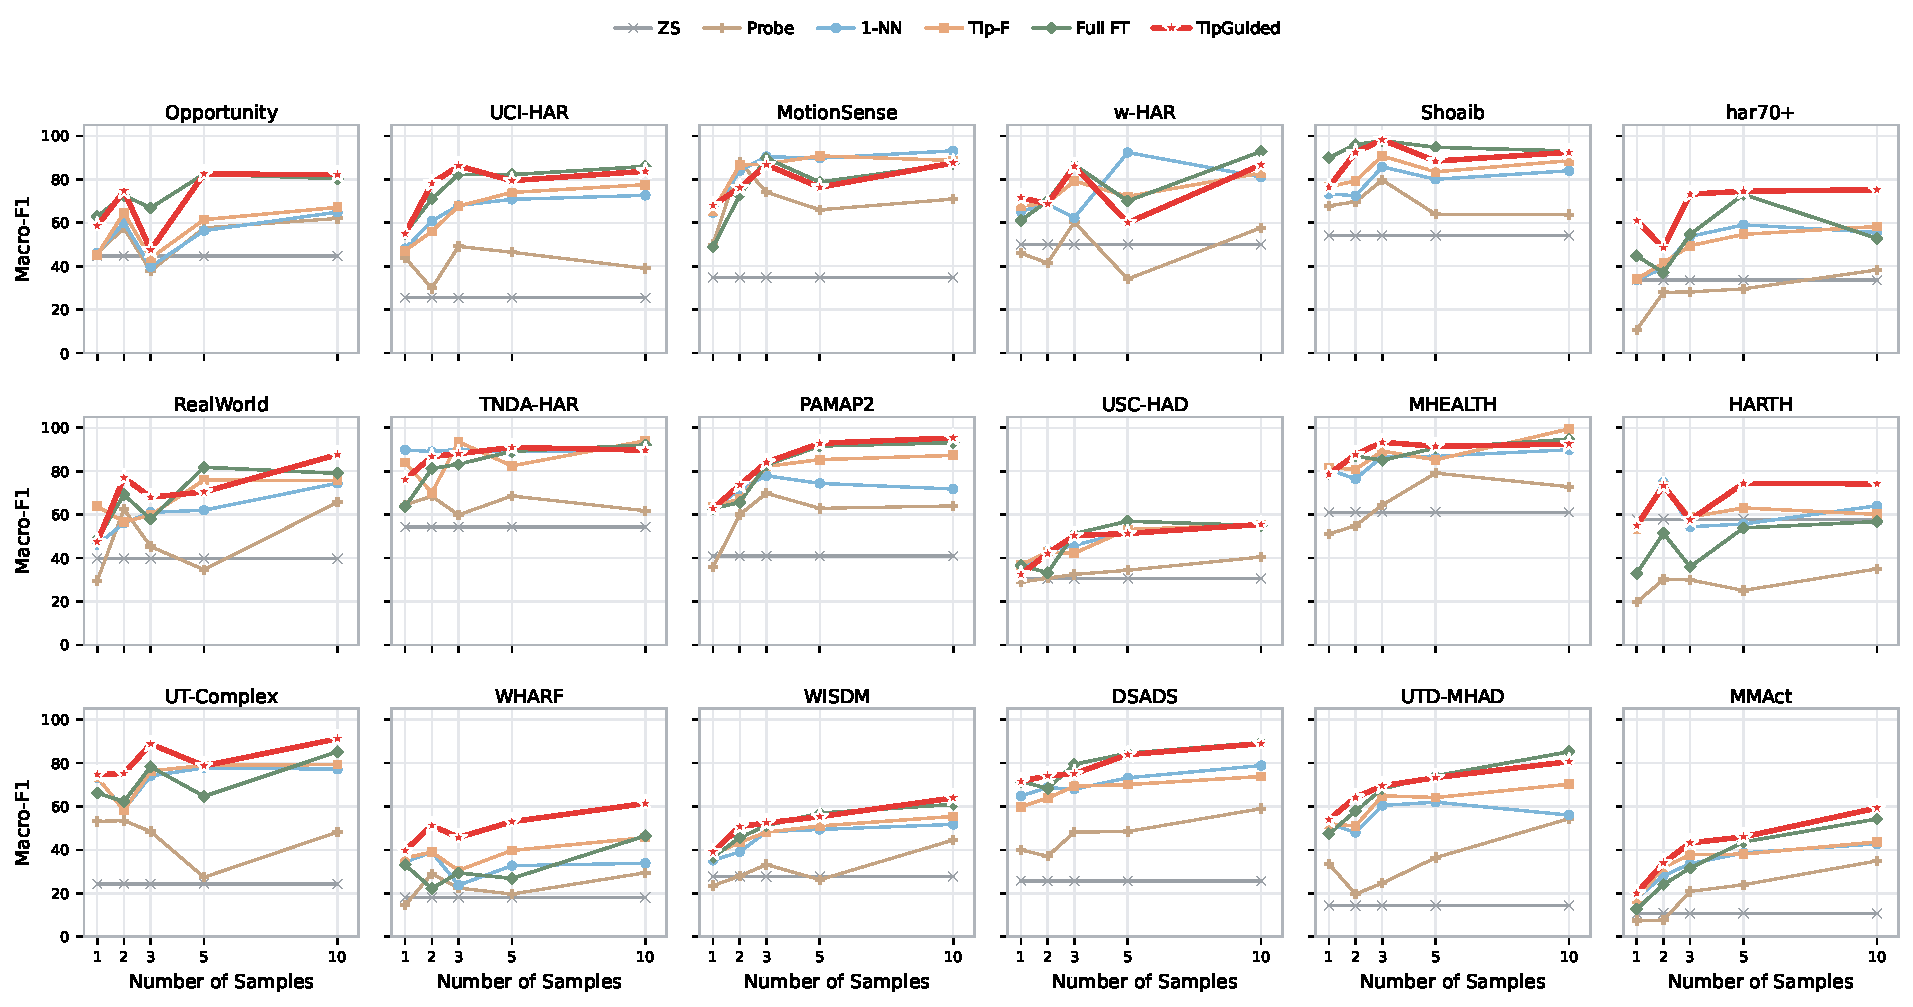
\includegraphics[width=\linewidth]{fig_fewshot_panel_f1.pdf}
\caption{\textbf{Few-shot fine-tuning results (Macro-F1).}
Layout mirrors UniMTS Fig.~4 on the same 18 datasets and \(k\in\{1,2,3,5,10\}\).
Curves are our runs; TipGuided is highlighted in red.}
\label{fig:panel}
\end{figure}

\begin{table}[t]
\centering
\caption{Few-shot averages on 18 datasets (official UniMTS indices; our runs).
Acc / Macro-F1 in \%. Best per \(k\) in \textbf{bold}.}
\label{tab:main}
\small
\setlength{\tabcolsep}{3.5pt}
\begin{tabular}{lcccccc}
\toprule
\(k\) & ZS & 1-NN & Probe & Tip-F & Full FT & \textbf{TipGuided} \\
\midrule
1
  & 44.4/36.0 & 57.8/54.3 & 45.8/37.0 & 59.0/55.3 & 61.2/53.0
  & \textbf{63.0/57.9} \\
2
  & 44.4/36.0 & 63.0/59.9 & 53.0/44.2 & 63.2/59.8 & 67.8/60.4
  & \textbf{71.6/68.2} \\
3
  & 44.4/36.0 & 65.0/62.5 & 54.6/46.1 & 67.6/65.1 & 72.8/67.4
  & \textbf{74.6/71.9} \\
5
  & 44.4/36.0 & 68.6/66.8 & 51.9/43.6 & 70.5/68.0 & 78.0/72.0
  & \textbf{78.4/73.5} \\
10
  & 44.4/36.0 & 70.6/68.7 & 61.5/52.3 & 75.1/72.4 & 81.5/76.9
  & \textbf{83.2/80.5} \\
\bottomrule
\end{tabular}
\end{table}

\begin{figure}[t]
\centering
\begin{subfigure}{0.56\linewidth}
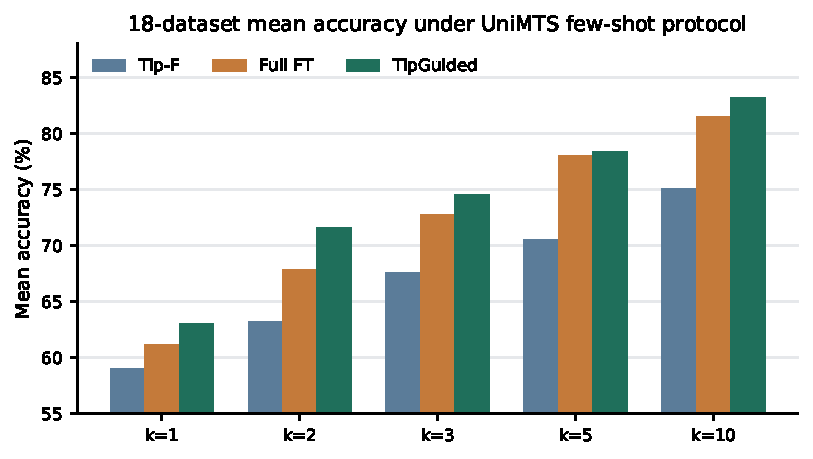
\includegraphics[width=\linewidth]{fig_main_bars.pdf}
\caption{Mean accuracy.}
\label{fig:mainbars}
\end{subfigure}
\hfill
\begin{subfigure}{0.42\linewidth}
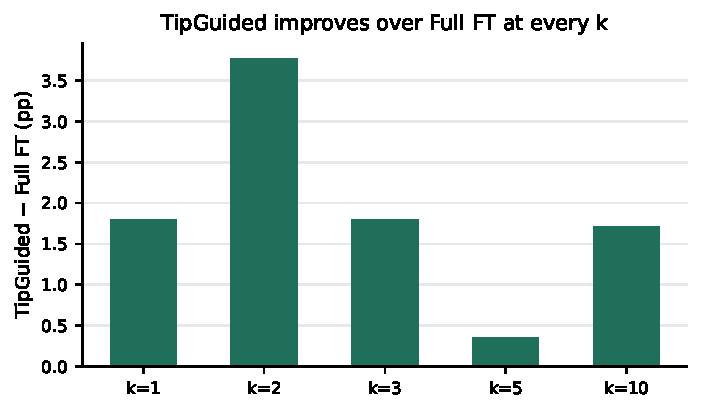
\includegraphics[width=\linewidth]{fig_delta_full.pdf}
\caption{Gap vs Full FT.}
\label{fig:delta}
\end{subfigure}
\caption{\textbf{Aggregate few-shot accuracy.}
TipGuided exceeds Full FT at every \(k\).}
\label{fig:main}
\end{figure}

\subsection{Full-shot context (reported)}
Table~\ref{tab:full-reported} reproduces UniMTS Table~2 averages.
Full-shot uses the entire target training split and is an upper reference for the same cross-dataset benchmark; our few-shot TipGuided at \(k{=}10\) reaches \(83.2\) Acc, closing much of the gap to reported UniMTS full-shot (\(90.6\)).

\begin{table}[t]
\centering
\caption{Full-shot averages on 18 datasets $^\dagger$ (UniMTS Table~2).
Best in \textbf{bold}.}
\label{tab:full-reported}
\small
\setlength{\tabcolsep}{3.2pt}
\begin{tabular}{lcc}
\toprule
Method & Acc (\%) & Macro-F1 (\%) \\
\midrule
ImageBind$^\dagger$ & 85.0 & 78.1 \\
IMU2CLIP$^\dagger$ & 80.5 & 75.0 \\
TST$^\dagger$ & 79.9 & 74.2 \\
TARNet$^\dagger$ & 75.1 & 65.9 \\
TS2Vec$^\dagger$ & 84.5 & 79.8 \\
BioBankSSL$^\dagger$ & 85.8 & 82.7 \\
THAT$^\dagger$ & 80.1 & 74.5 \\
IMUGPT$^\dagger$ & 74.4 & 66.4 \\
TimesNet$^\dagger$ & 78.0 & 72.6 \\
GPT4TS$^\dagger$ & 78.7 & 72.5 \\
SHARE$^\dagger$ & 85.8 & 80.1 \\
Random$^\dagger$ & 84.7 & 78.5 \\
\textbf{UniMTS}$^\dagger$ & \textbf{90.6} & \textbf{87.5} \\
\bottomrule
\end{tabular}
\end{table}

\subsection{Diagnostic ladder}
Figure~\ref{fig:ladder} orders methods at \(k{=}5\).
Zero-shot and linear probes sit far below Tip-F, confirming that cache adaptation exploits support geometry beyond a linear head.
Tip+ barely moves Tip-F, marking frozen saturation.
Full FT jumps into the high \(0.78\) range; TipGuided clears that bar.

\begin{figure}[t]
\centering
\begin{subfigure}{0.48\linewidth}
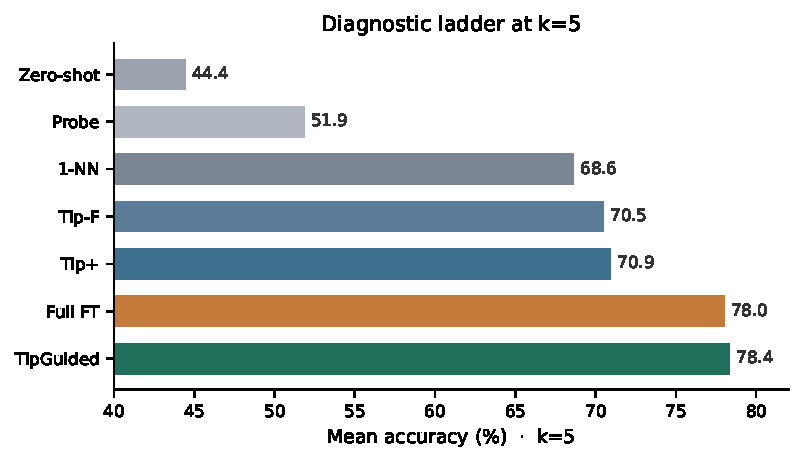
\includegraphics[width=\linewidth]{fig_ladder_k5.pdf}
\caption{Method ladder at \(k{=}5\).}
\label{fig:ladder}
\end{subfigure}
\hfill
\begin{subfigure}{0.48\linewidth}
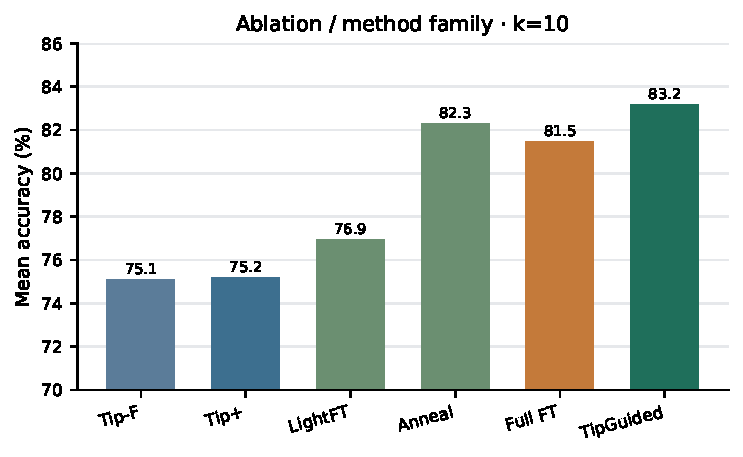
\includegraphics[width=\linewidth]{fig_ablation_k10.pdf}
\caption{Method family at \(k{=}10\).}
\label{fig:ablation}
\end{subfigure}
\caption{\textbf{Where gains come from.}
Frozen Tip saturates; encoder updates with Tip priors deliver the remaining lift.}
\end{figure}

\subsection{Per-dataset behavior}
Figure~\ref{fig:heat} compares Tip-F, Full FT, and TipGuided on each dataset.
At \(k{=}10\), TipGuided wins on \(12/18\) datasets, with large gains on w-HAR, Wharf, ut-complex, MMAct, and realworld---settings where prior-free FT overfits heterogeneous or smaller targets.
At \(k{=}5\), TipGuided still trails Full FT on Shoaib, realworld, and USCHAD, while leading on Wharf, UTD-MHAD, and MMAct; the mean remains higher because wins concentrate on hard, low-resource targets.

\begin{figure}[t]
\centering
\begin{subfigure}{0.42\linewidth}
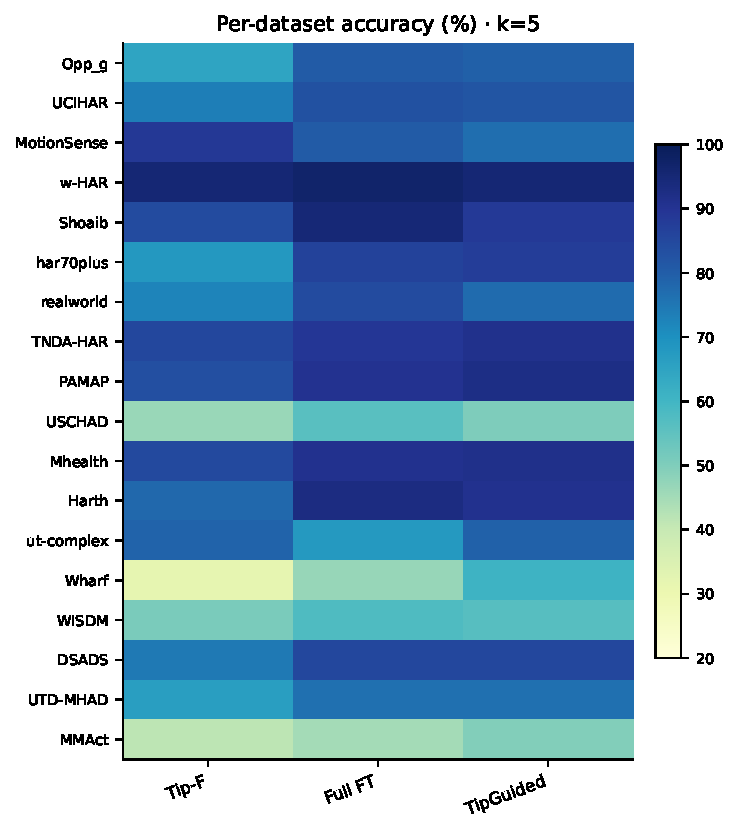
\includegraphics[width=\linewidth]{fig_heatmap_k5.pdf}
\caption{Per-dataset accuracy, \(k{=}5\).}
\end{subfigure}
\hfill
\begin{subfigure}{0.55\linewidth}
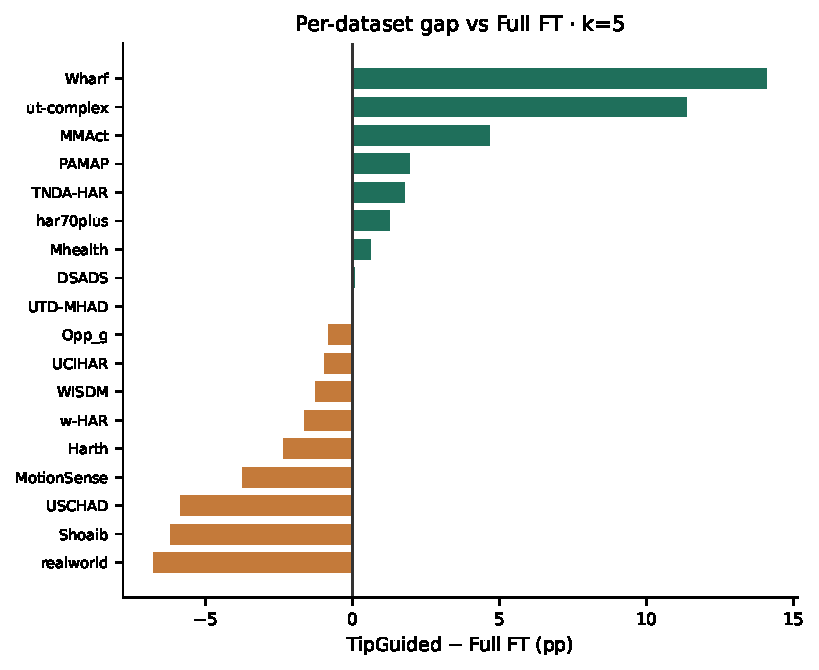
\includegraphics[width=\linewidth]{fig_gap_datasets_k5.pdf}
\caption{TipGuided $-$ Full FT, \(k{=}5\).}
\end{subfigure}
\caption{\textbf{Dataset-level view.}
TipGuided concentrates gains where Full FT overfits.}
\label{fig:heat}
\end{figure}

\subsection{Training dynamics}
Figure~\ref{fig:tipfloss} shows Tip-F key training: support CE drops quickly while test accuracy plateaus---the frozen encoder never moves.
Figure~\ref{fig:traincmp} contrasts Full FT and TipGuided on matched supports and budgets.
TipGuided starts from a much stronger test accuracy because Tip/text logits are available from epoch~0, and its fused objective drives support CE down faster than CE-only Full FT.
On UCIHAR and PAMAP, TipGuided remains competitive throughout; on Wharf the short-horizon curve is noisier, consistent with that dataset's small test pool.
The 18-dataset means in Table~\ref{tab:main} aggregate these trajectories under the full training recipe.

\begin{figure}[t]
\centering
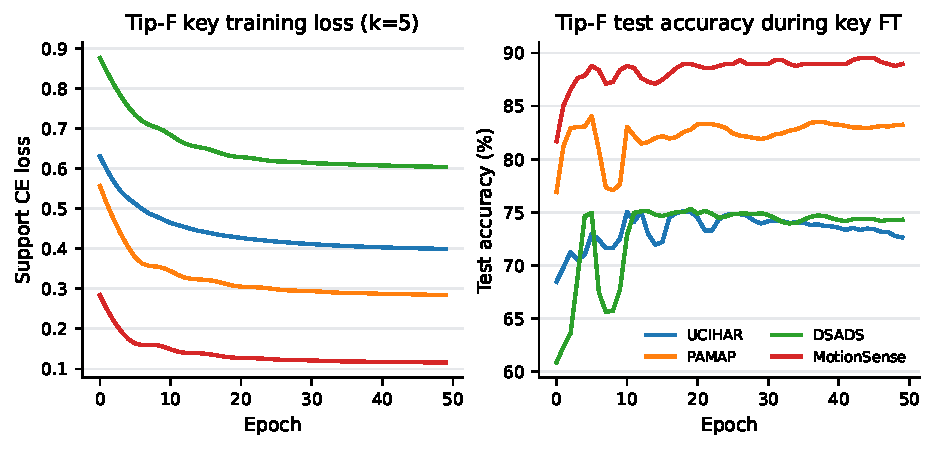
\includegraphics[width=0.92\linewidth]{fig_tipf_loss.pdf}
\caption{\textbf{Frozen Tip-F dynamics} (\(k{=}5\)).
Key fine-tuning fits the support set, yet test accuracy saturates---the encoder never moves.}
\label{fig:tipfloss}
\end{figure}

\begin{figure}[t]
\centering
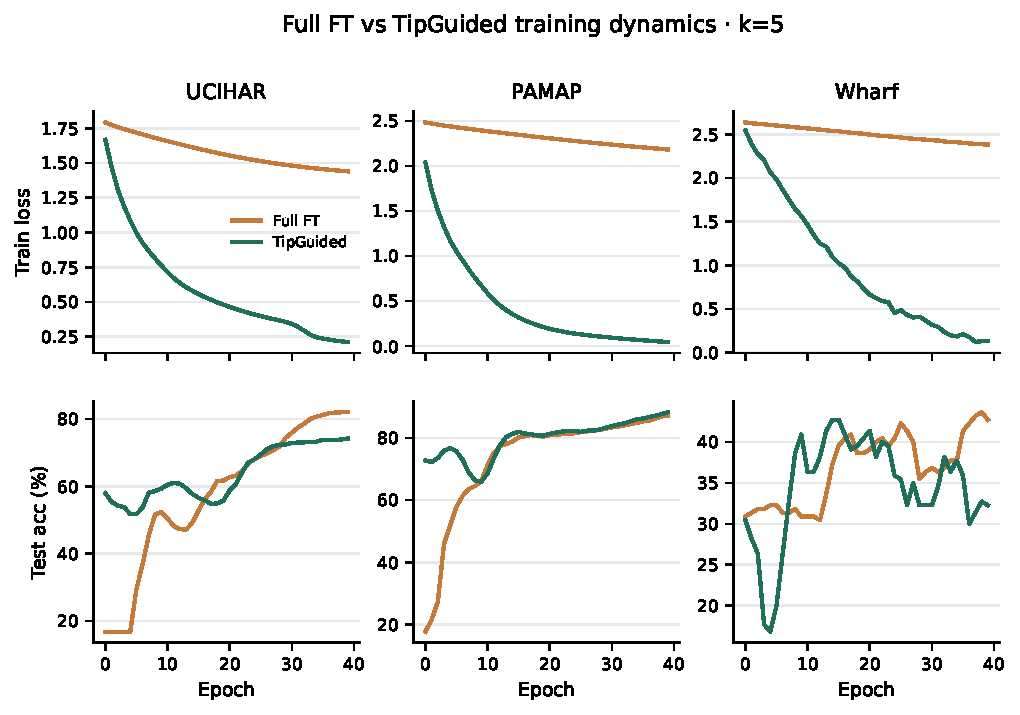
\includegraphics[width=\linewidth]{fig_train_compare.pdf}
\caption{\textbf{Full FT vs TipGuided training} (\(k{=}5\), 40 epochs).
TipGuided enters with higher test accuracy from Tip/text priors and reduces support CE faster via the fused objective.}
\label{fig:traincmp}
\end{figure}

\subsection{Feature geometry}
Figure~\ref{fig:tsne} visualizes t-SNE of test embeddings before and after TipGuided-CE on representative datasets.
After adaptation, class clusters tighten and inter-class gaps widen relative to the frozen UniMTS features, matching the accuracy gains in Table~\ref{tab:main}.

\begin{figure}[t]
\centering
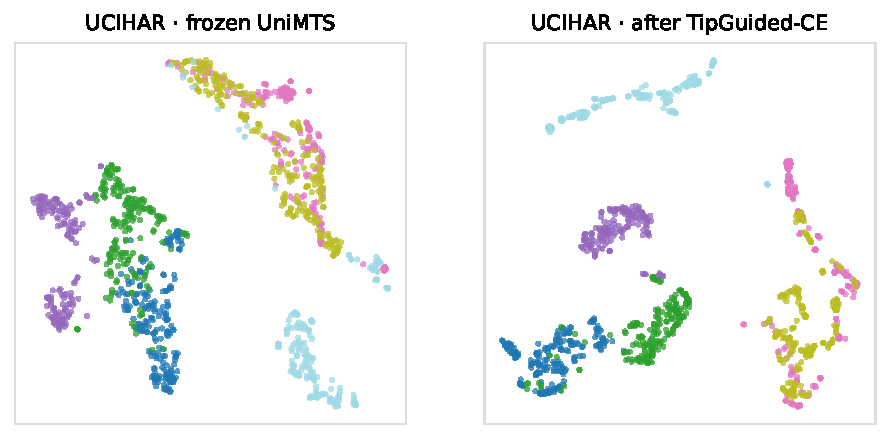
\includegraphics[width=0.95\linewidth]{fig_tsne_UCIHAR.pdf}\\[0.35em]
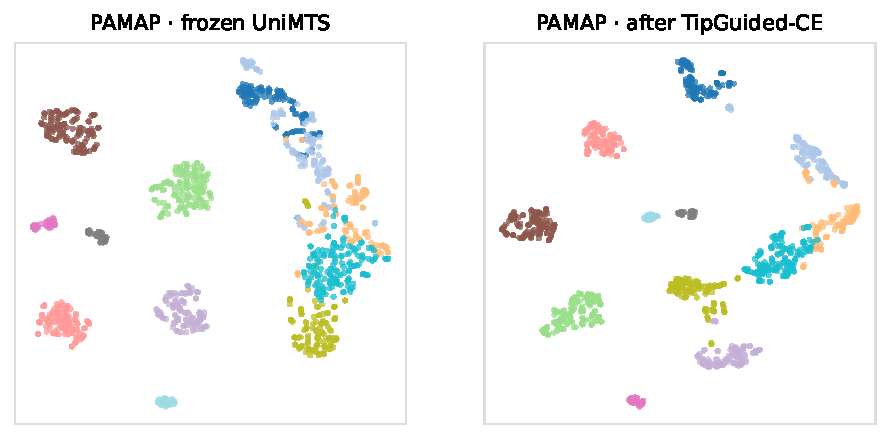
\includegraphics[width=0.95\linewidth]{fig_tsne_PAMAP.pdf}\\[0.35em]
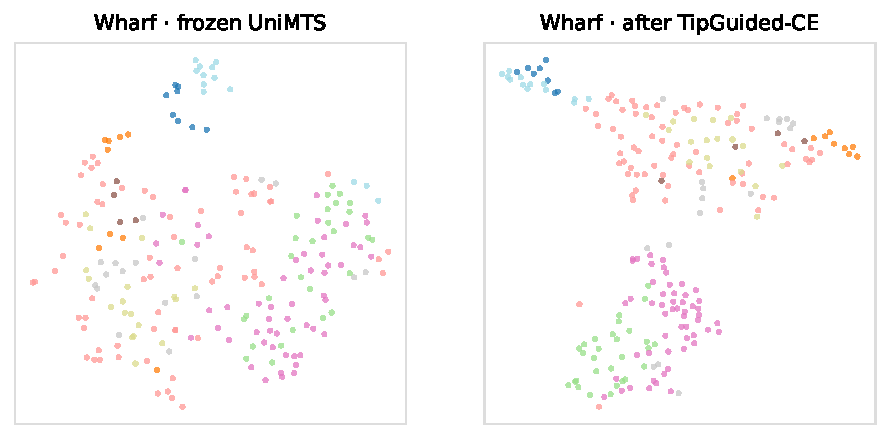
\includegraphics[width=0.95\linewidth]{fig_tsne_Wharf.pdf}
\caption{\textbf{t-SNE of test features} (\(k{=}5\)).
Each row: frozen UniMTS (left) vs TipGuided-CE (right) for UCIHAR, PAMAP, and Wharf.
TipGuided tightens class clusters and widens inter-class gaps.}
\label{fig:tsne}
\end{figure}

\subsection{Ablations}
At \(k{=}10\) (Figure~\ref{fig:ablation}), LightFT and Tip\(\rightarrow\)CE annealing improve over Tip-F yet remain below TipGuided CE (\(0.832\)).
Longer aggressive schedules without Tip structure do not substitute for the prior: a longer CE-only TipGuided run at \(k{=}10\) underperforms the default 100-epoch recipe.

% ============================================================
\section{Discussion}
\label{sec:disc}

TipGuided reframes Tip-Adapter from a frozen classifier into an adaptation prior for encoder fine-tuning.
The central empirical fact is simple: under UniMTS's cross-dataset few-shot protocol, keeping Tip/text geometry while updating the motion encoder beats discarding that geometry (Full FT) and beats refusing to update the encoder (Tip-F).

The \(k\)-dependent recipe is itself informative.
When supports are extremely sparse, Tip logits supply supervision the CE head cannot yet estimate---hence the large early-epoch gap in Figure~\ref{fig:traincmp}.
When supports grow, CE-primary decoding dominates and Tip mainly shapes the adaptation trajectory.

\paragraph{Scope.}
All numbers use UniMTS checkpoints and official splits.
Extending TipGuided to other IMU foundation models, confirming the tight \(k{=}5\) margin with multiple seeds, and collapsing fuse/CE-primary into one tip-weight schedule are concrete follow-ups.

% ============================================================
\section{Conclusion}
\label{sec:conc}

Cross-dataset few-shot HAR exposes a clear failure mode of both frozen Tip caches and prior-free full fine-tuning.
TipGuided closes that gap by fine-tuning UniMTS under Tip-cache and text priors, improving mean accuracy over Full FT for every official \(k\) on 18 datasets.
Adaptation should update the encoder while keeping foundation-model geometry explicit.

% ============================================================
\section*{Acknowledgments}
[Anonymous.]

% ============================================================
\bibliographystyle{plain}
\begin{thebibliography}{99}

\bibitem{unimts}
Xiyuan~Zhang, Diyan~Teng, Ranak~Roy~Chowdhury, Shuheng~Li, Dezhi~Hong, Rajesh~K.~Gupta, and Jingbo~Shang.
\newblock UniMTS: Unified Pre-training for Motion Time Series.
\newblock In {\em NeurIPS}, 2024.

\bibitem{tipadapter}
Zhang~et~al.
\newblock Tip-Adapter: Training-free Adaption of CLIP for Few-shot Classification.
\newblock In {\em ECCV}, 2022.

\bibitem{clip}
Radford~et~al.
\newblock Learning Transferable Visual Models From Natural Language Supervision.
\newblock In {\em ICML}, 2021.

\bibitem{stgcn}
Yan, Xiong, and Lin.
\newblock Spatial Temporal Graph Convolutional Networks for Skeleton-Based Action Recognition.
\newblock In {\em AAAI}, 2018.

\bibitem{protonet}
Snell, Swersky, and Zemel.
\newblock Prototypical Networks for Few-shot Learning.
\newblock In {\em NeurIPS}, 2017.

\end{thebibliography}

\end{document}
